\documentclass{standalone}
\usepackage{tikz}
\usetikzlibrary{patterns, positioning}
\usepackage[sfdefault]{ClearSans} %% option 'sfdefault' activates Clear Sans as the default text font
\usepackage[T1]{fontenc}

\begin{document}
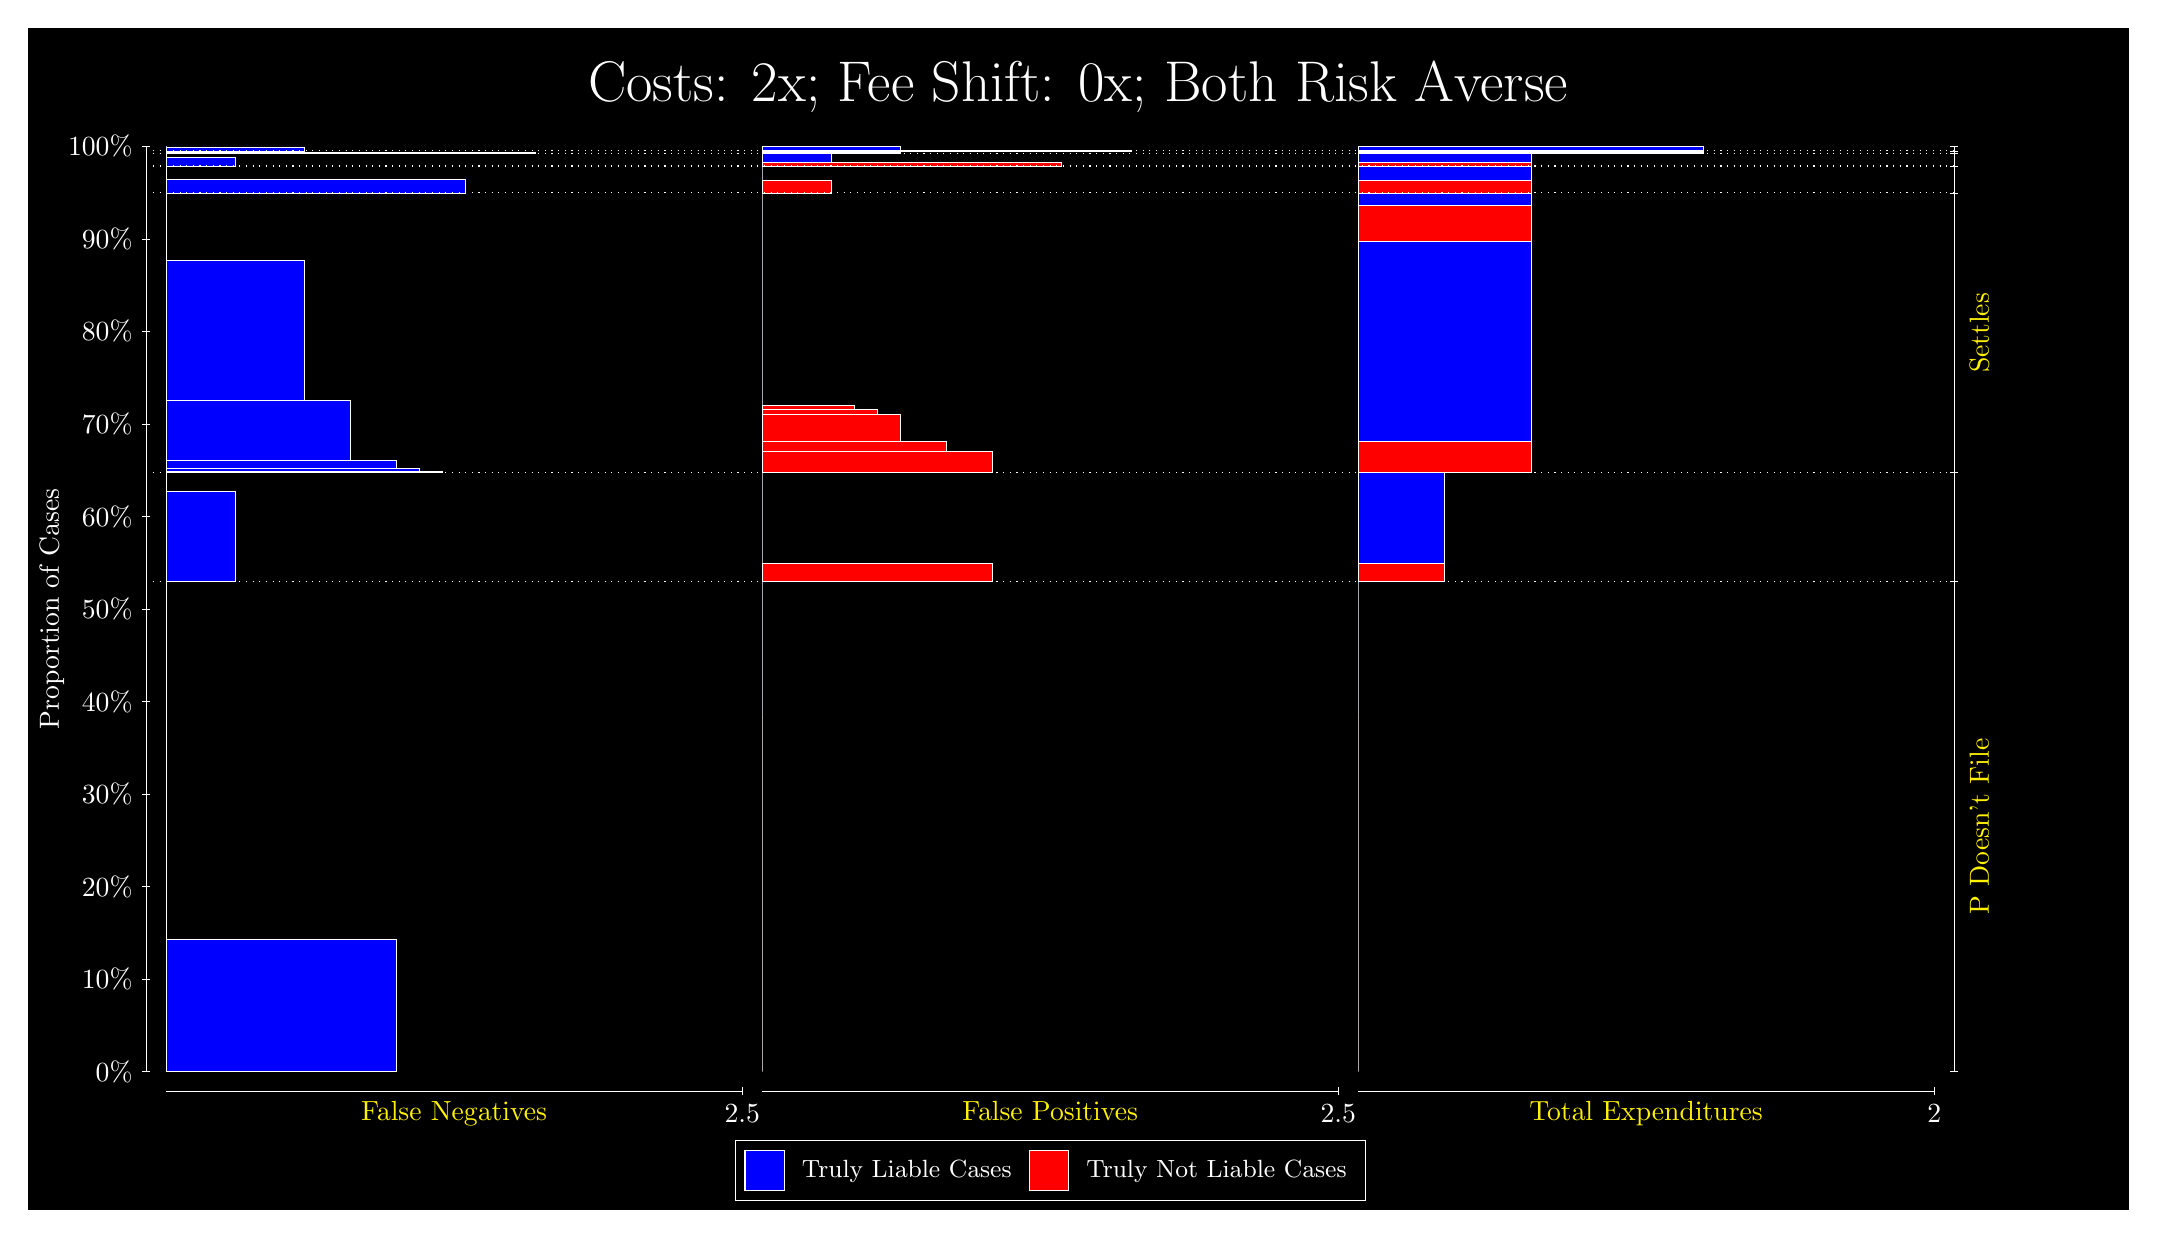
\begin{tikzpicture}
\draw[fill=black] (0,0) rectangle (26.667,15);
\draw[text=white] (0,13.5) rectangle (26.667,15) node[midway] {\huge Costs: 2x; Fee Shift: 0x; Both Risk Averse};
\draw[white, very thin] (1.5,1.75) -- (1.5,13.5);
\node[rotate=90, text=white, anchor=center] at (0.3, 7.625) {Proportion of Cases};
\draw[white, very thin] (1.45,1.75) -- (1.55,1.75);
\node[text=white, anchor=east] at (1.45, 1.75) {0\%};
\draw[white, very thin] (1.45,2.925) -- (1.55,2.925);
\node[text=white, anchor=east] at (1.45, 2.925) {10\%};
\draw[white, very thin] (1.45,4.1) -- (1.55,4.1);
\node[text=white, anchor=east] at (1.45, 4.1) {20\%};
\draw[white, very thin] (1.45,5.275) -- (1.55,5.275);
\node[text=white, anchor=east] at (1.45, 5.275) {30\%};
\draw[white, very thin] (1.45,6.45) -- (1.55,6.45);
\node[text=white, anchor=east] at (1.45, 6.45) {40\%};
\draw[white, very thin] (1.45,7.625) -- (1.55,7.625);
\node[text=white, anchor=east] at (1.45, 7.625) {50\%};
\draw[white, very thin] (1.45,8.8) -- (1.55,8.8);
\node[text=white, anchor=east] at (1.45, 8.8) {60\%};
\draw[white, very thin] (1.45,9.975) -- (1.55,9.975);
\node[text=white, anchor=east] at (1.45, 9.975) {70\%};
\draw[white, very thin] (1.45,11.15) -- (1.55,11.15);
\node[text=white, anchor=east] at (1.45, 11.15) {80\%};
\draw[white, very thin] (1.45,12.325) -- (1.55,12.325);
\node[text=white, anchor=east] at (1.45, 12.325) {90\%};
\draw[white, very thin] (1.45,13.5) -- (1.55,13.5);
\node[text=white, anchor=east] at (1.45, 13.5) {100\%};

\draw[white, very thin] (24.457,1.75) -- (24.457,13.5);
\draw[white, very thin] (24.407,1.75) -- (24.507,1.75);
\node[anchor=west] at (24.407, 1.75) {};
\draw[white, very thin] (24.407,7.9724) -- (24.507,7.9724);
\node[anchor=west] at (24.407, 7.9724) {};
\draw[white, very thin] (24.407,9.3541) -- (24.507,9.3541);
\node[anchor=west] at (24.407, 9.3541) {};
\draw[white, very thin] (24.407,12.909) -- (24.507,12.909);
\node[anchor=west] at (24.407, 12.909) {};
\draw[white, very thin] (24.407,13.25) -- (24.507,13.25);
\node[anchor=west] at (24.407, 13.25) {};
\draw[white, very thin] (24.407,13.41) -- (24.507,13.41);
\node[anchor=west] at (24.407, 13.41) {};
\draw[white, very thin] (24.407,13.442) -- (24.507,13.442);
\node[anchor=west] at (24.407, 13.442) {};
\draw[white, very thin] (24.407,13.5) -- (24.507,13.5);
\node[anchor=west] at (24.407, 13.5) {};

\draw[white, very thin, fill=blue] (1.75,1.75) rectangle (4.6775,3.4358);
\draw[white, very thin, fill=red] (1.75,3.4358) rectangle (1.75,7.9724);
\draw[white, very thin, fill=blue] (1.75,7.9724) rectangle (2.6283,9.1191);
\draw[white, very thin, fill=red] (1.75,9.1191) rectangle (1.75,9.3541);
\draw[white, very thin, fill=blue] (1.75,9.3541) rectangle (5.2631,9.3766);
\draw[white, very thin, fill=blue] (1.75,9.3766) rectangle (4.9703,9.4129);
\draw[white, very thin, fill=blue] (1.75,9.4129) rectangle (4.6775,9.5074);
\draw[white, very thin, fill=blue] (1.75,9.5074) rectangle (4.092,10.272);
\draw[white, very thin, fill=blue] (1.75,10.272) rectangle (3.5065,12.055);
\draw[white, very thin, fill=red] (1.75,12.055) rectangle (1.75,12.909);
\draw[white, very thin, fill=blue] (1.75,12.909) rectangle (5.5558,13.084);
\draw[white, very thin, fill=red] (1.75,13.084) rectangle (1.75,13.25);
\draw[white, very thin, fill=blue] (1.75,13.25) rectangle (2.6283,13.358);
\draw[white, very thin, fill=red] (1.75,13.358) rectangle (1.75,13.41);
\draw[white, very thin, fill=blue] (1.75,13.41) rectangle (6.4341,13.423);
\draw[white, very thin, fill=red] (1.75,13.423) rectangle (1.75,13.442);
\draw[white, very thin, fill=blue] (1.75,13.442) rectangle (3.5065,13.486);
\draw[white, very thin, fill=red] (1.75,13.486) rectangle (1.75,13.5);
\draw[white, very thin, fill=red] (9.3189,1.75) rectangle (9.3189,6.2867);
\draw[white, very thin, fill=blue] (9.3189,6.2867) rectangle (9.3189,7.9724);
\draw[white, very thin, fill=red] (9.3189,7.9724) rectangle (12.246,8.2075);
\draw[white, very thin, fill=blue] (9.3189,8.2075) rectangle (9.3189,9.3541);
\draw[white, very thin, fill=red] (9.3189,9.3541) rectangle (12.246,9.6312);
\draw[white, very thin, fill=red] (9.3189,9.6312) rectangle (11.661,9.75);
\draw[white, very thin, fill=red] (9.3189,9.75) rectangle (11.075,10.091);
\draw[white, very thin, fill=red] (9.3189,10.091) rectangle (10.783,10.156);
\draw[white, very thin, fill=red] (9.3189,10.156) rectangle (10.49,10.208);
\draw[white, very thin, fill=blue] (9.3189,10.208) rectangle (9.3189,12.909);
\draw[white, very thin, fill=red] (9.3189,12.909) rectangle (10.197,13.075);
\draw[white, very thin, fill=blue] (9.3189,13.075) rectangle (9.3189,13.25);
\draw[white, very thin, fill=red] (9.3189,13.25) rectangle (13.125,13.301);
\draw[white, very thin, fill=blue] (9.3189,13.301) rectangle (10.197,13.41);
\draw[white, very thin, fill=red] (9.3189,13.41) rectangle (11.075,13.428);
\draw[white, very thin, fill=blue] (9.3189,13.428) rectangle (9.3189,13.442);
\draw[white, very thin, fill=red] (9.3189,13.442) rectangle (14.003,13.456);
\draw[white, very thin, fill=blue] (9.3189,13.456) rectangle (11.075,13.5);
\draw[white, very thin, fill=red] (16.888,1.75) rectangle (16.888,6.2867);
\draw[white, very thin, fill=blue] (16.888,6.2867) rectangle (16.888,7.9724);
\draw[white, very thin, fill=red] (16.888,7.9724) rectangle (17.986,8.2075);
\draw[white, very thin, fill=blue] (16.888,8.2075) rectangle (17.986,9.3541);
\draw[white, very thin, fill=red] (16.888,9.3541) rectangle (19.083,9.75);
\draw[white, very thin, fill=blue] (16.888,9.75) rectangle (19.083,12.298);
\draw[white, very thin, fill=red] (16.888,12.298) rectangle (19.083,12.755);
\draw[white, very thin, fill=blue] (16.888,12.755) rectangle (19.083,12.909);
\draw[white, very thin, fill=red] (16.888,12.909) rectangle (19.083,13.075);
\draw[white, very thin, fill=blue] (16.888,13.075) rectangle (19.083,13.25);
\draw[white, very thin, fill=red] (16.888,13.25) rectangle (19.083,13.301);
\draw[white, very thin, fill=blue] (16.888,13.301) rectangle (19.083,13.41);
\draw[white, very thin, fill=red] (16.888,13.41) rectangle (21.279,13.428);
\draw[white, very thin, fill=blue] (16.888,13.428) rectangle (21.279,13.442);
\draw[white, very thin, fill=red] (16.888,13.442) rectangle (21.279,13.456);
\draw[white, very thin, fill=blue] (16.888,13.456) rectangle (21.279,13.5);
\draw[white, dotted] (1.5,7.9724) -- (24.457,7.9724);
\draw[white, dotted] (1.5,9.3541) -- (24.457,9.3541);
\draw[white, dotted] (1.5,12.909) -- (24.457,12.909);
\draw[white, dotted] (1.5,13.25) -- (24.457,13.25);
\draw[white, dotted] (1.5,13.41) -- (24.457,13.41);
\draw[white, dotted] (1.5,13.442) -- (24.457,13.442);
\draw[white, very thin] (1.75,1.5) -- (9.0689,1.5);
\node[text=yellow, anchor=north] at (5.4094, 1.5) {False Negatives};
\draw[white, very thin] (9.0689,1.45) -- (9.0689,1.55);
\node[text=white, anchor=north] at (9.0689, 1.45) {2.5};

\draw[white, very thin] (9.3189,1.5) -- (16.638,1.5);
\node[text=yellow, anchor=north] at (12.978, 1.5) {False Positives};
\draw[white, very thin] (16.638,1.45) -- (16.638,1.55);
\node[text=white, anchor=north] at (16.638, 1.45) {2.5};

\draw[white, very thin] (16.888,1.5) -- (24.207,1.5);
\node[text=yellow, anchor=north] at (20.547, 1.5) {Total Expenditures};
\draw[white, very thin] (24.207,1.45) -- (24.207,1.55);
\node[text=white, anchor=north] at (24.207, 1.45) {2};

\node[text=yellow, centered, rotate=90] at (24.777, 4.8612) {P Doesn't File};

\node[text=yellow, centered, rotate=90] at (24.777, 11.131) {Settles};





\draw (12.978300999999998,1.5) node[draw=none] (baseCoordinate) {};
\begin{scope}[align=center]
        \matrix[scale=0.5, draw=white, below=0.5cm of baseCoordinate, nodes={draw}, column sep=0.1cm]{
            \node[rectangle, draw, minimum width=0.5cm, minimum height=0.5cm, fill=blue] {}; &
            \node[draw=none, font=\small, text=white] (B) {Truly Liable Cases}; &
            \node[rectangle, draw, minimum width=0.5cm, minimum height=0.5cm, fill=red] {}; &
            \node[draw=none, font=\small, text=white] (B) {Truly Not Liable Cases}; \\
            };
\end{scope}

\end{tikzpicture}
\end{document}